\section[Feature Spaces in Machine Learning]{Sidebar: Feature Spaces in Machine Learning}\label{sb:featspace}
Suppose we have data $\sampSetClass = \sampSetClassLong$, where $x_i\in\domI$ and $y_i\in\domO$. Here, $\domI$ is the input domain (state space), and 
is generally a subset of $\R^D$, although more general sets such as discrete spaces, graphs, or text documents can be considered.
Similarly, $\domO$, the output domain, can be just as general as $\domI$. Control theorists are most likely familiar with 
input-output pairs where $x_i\in\R^N$ and $y_i$ is either in $\R$ or $\R^M$. In machine learning, our goal is typically to solve for a function
$f$ that minimizes a \emph{loss function} $L(f, \sampSetClass)\mapsto\R$, which measures the error between a prediction $f(x_i)$ given a datapoint $x_i$, and $y_i$, averaged over the entire dataset $\sampSetClass$. A concrete example of this will be given shortly.
Different loss functions result in different algorithms to solve these problems. Similarly, different choices of the spaces where $f$ arises from also 
result in different algorithms and techniques, and sometimes form entire subfields of machine learning. Generally, if $y_i$ are continuous, 
the task is called \emph{regression}, and if $y_i$ are discrete, the task is known as \emph{classification}. 

Just as in control theory, the design of the state space $\domI$ can be critical for the task we want to perform. Let's consider a simple
example. Suppose we have data from two \emph{classes} $\sampSetClass_A = \{(x_1^A, y_1^A), \dots, (x_N^A, y_N^A)\}$ and 
$\sampSetClass_B = \{(x_1^B, y_1^B), \dots, (x_N^B, y_N^B)\}$, where $x_i^{\{A,B\}}\in\R^D$, and $y_i^{\{A,B\}}\in\{-1,+1\}$, shown
in Figure \ref{fig:lisep_data}. Let $f$ be chosen from the class of linear algorithms, i.e. $f = w^Tx + b$, where $w\in\R^D, b\in\R$. 
We pick a loss $L$ that returns a loss of zero when the prediction is the correct class, and if the prediction is the incorrect class,
returns a higher value for misclassifications that are closer to the boundary. A classical example of such a loss is that used by
the perceptron algorithm, which can be written as 
\begin{align}\eqlabel{perc_loss}
 L(f, \sampSetClass) = \frac{1}{\nsamp}\sum_{i=1}^N\max(0, -y_iw^Tx). 
\end{align}
In general, the optimization problem solved in machine learning involves minimizing this loss subject to constraints. We can write this as
\begin{align}
 f^* = \argmin_{w,b} L(f, \sampSetClass) + \la g(f),
\end{align}
where $g$ represents some constraints on the function $f$. Equation \eqref{perc_loss} results in the famous \emph{perceptron algorithm},
which was one of the first machine learning algorithms, and the genesis of modern neural networks. 

Figure \ref{fig:linsep} shows a visual representation of where the perceptron algorithm can solve for the decision boundary with zero error. 
However, if the structure of the data has some nonlinearities, no solution will be found, as seen in Figure \ref{fig:nlinsep}. In this case,
the original space the data resides in is, in some sense, not a rich enough representation. If we could construct a mapping of the data to a
different space which gives a learning algorithm more degrees of freedom to work with, linear algorithms can still be deployed. 
If we map the same data using a nonlinear map $\phi(x,y):= (x^2, y^2, 2xy)$, the perceptron now finds a solution
in 3 dimensions, as seen in Figure \ref{fig:fmapped}. This example shows why so much of the work in machine learning focuses on 
learning the right representation for the data, for the right representation makes the classification task easy. Two major threads of 
research in the arena of feature maps over the last 40 years are decision trees, kernel methods, and neural networks, the latter
of which has gained remarkable notoriety in the last 10 years. Decision tree learning methods such as gradient boosting and random forests
arose from the statistics community and enjoy significant adoption in industry \cite{Wasserman}, but will not be described in detail in this work.  

\begin{figure}\label{fig:linsep}
\centering
    \subfloat[Data from classes $A$ and $B$.]
    {
    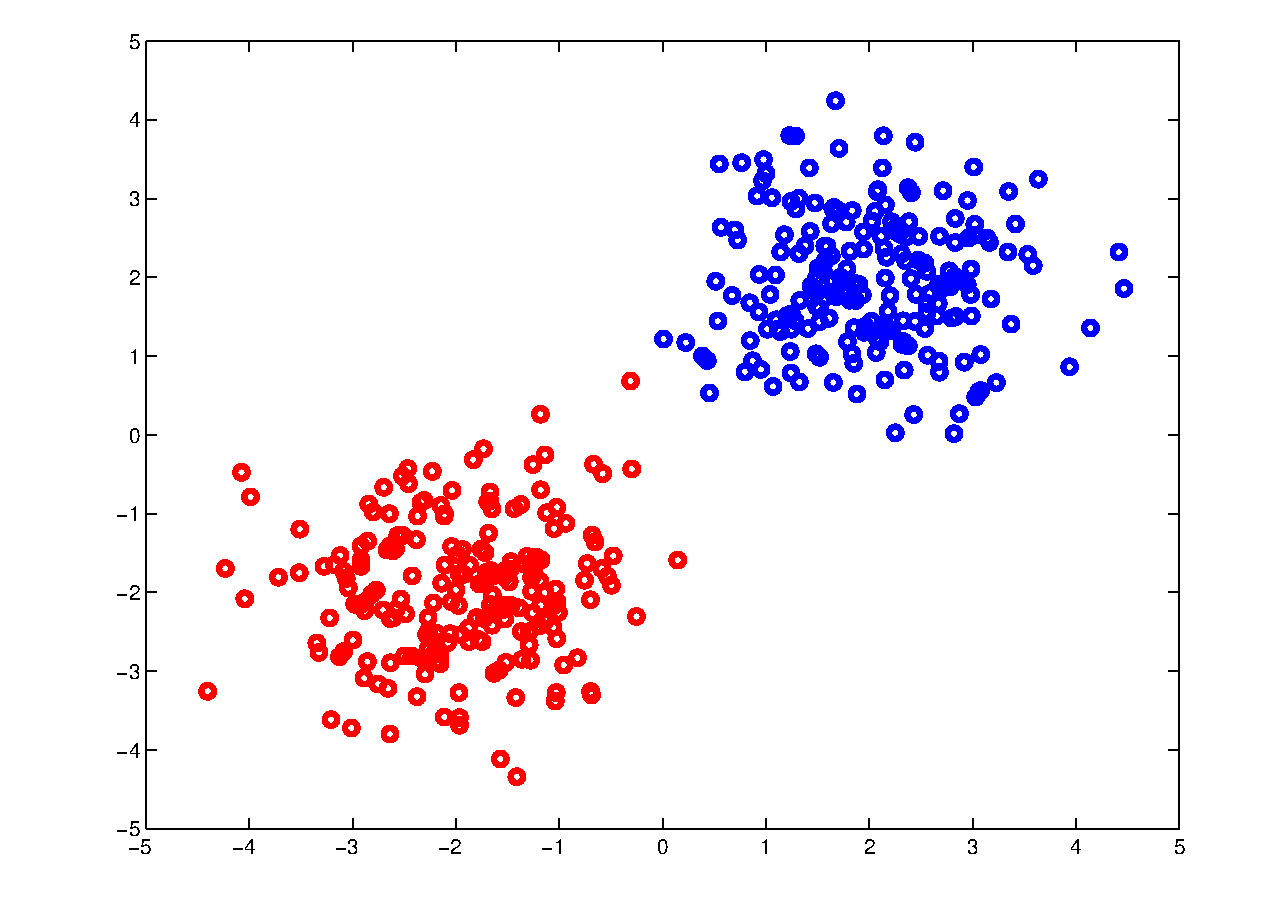
\includegraphics[width=0.45\columnwidth]{figures/linsep_data.pdf}
    \label{fig:lisep_data}}
     \subfloat[Linear boundary separating data.]
     {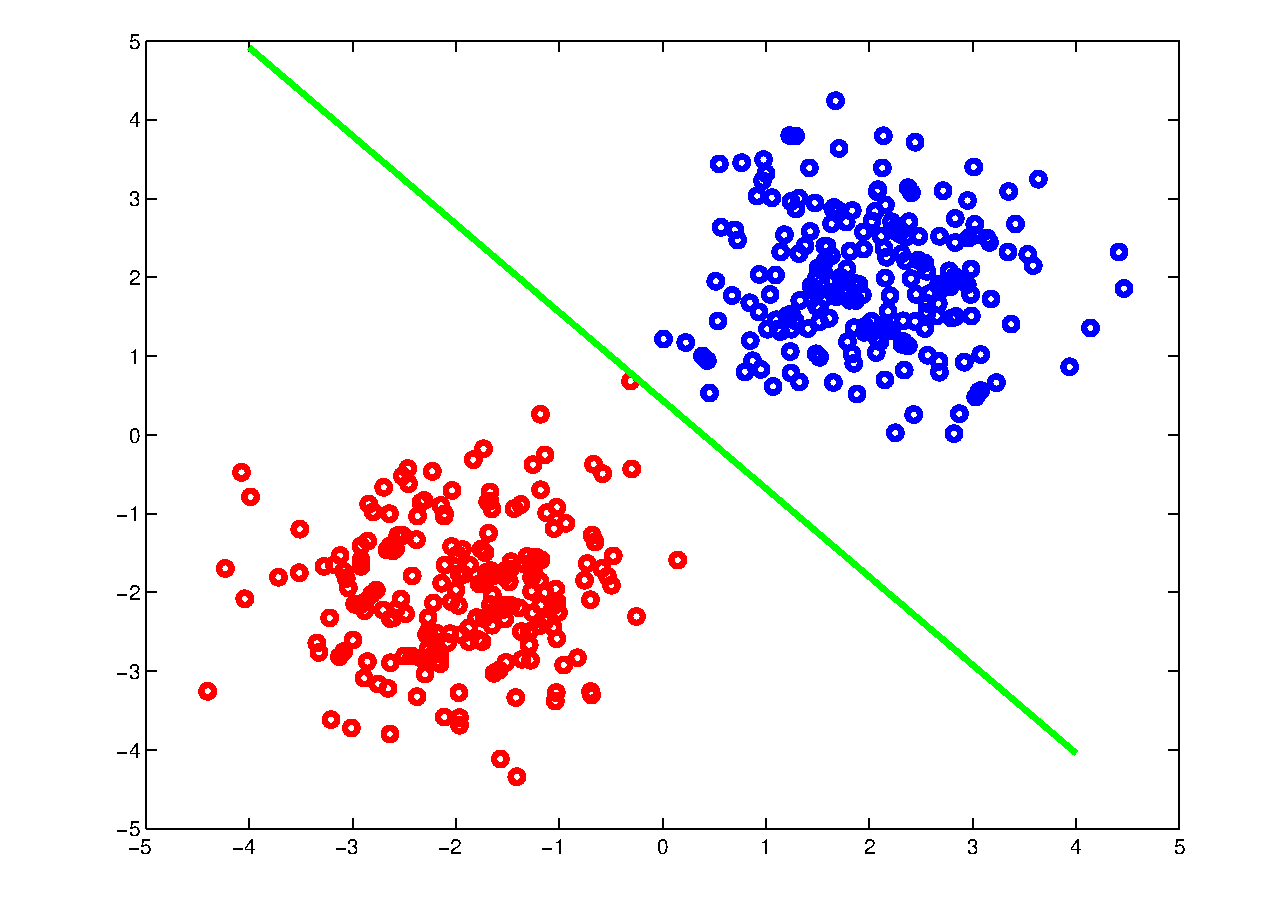
\includegraphics[width=0.45\columnwidth]{figures/linsep_data_perceptron.pdf}
     \label{fig:lin_sep_bound}}  
    \caption{Example of linearly separable data. Any simple linear learning algorithm e.g. perceptron, finds a solution.}
    \label{fig:linsep}
    %\end{figure}
%\begin{figure}[tbh] %{r}{0.5\textwidth}
\end{figure} 

\begin{figure}
\centering
    \subfloat[Data from classes $A$ and $B$.]
    {
    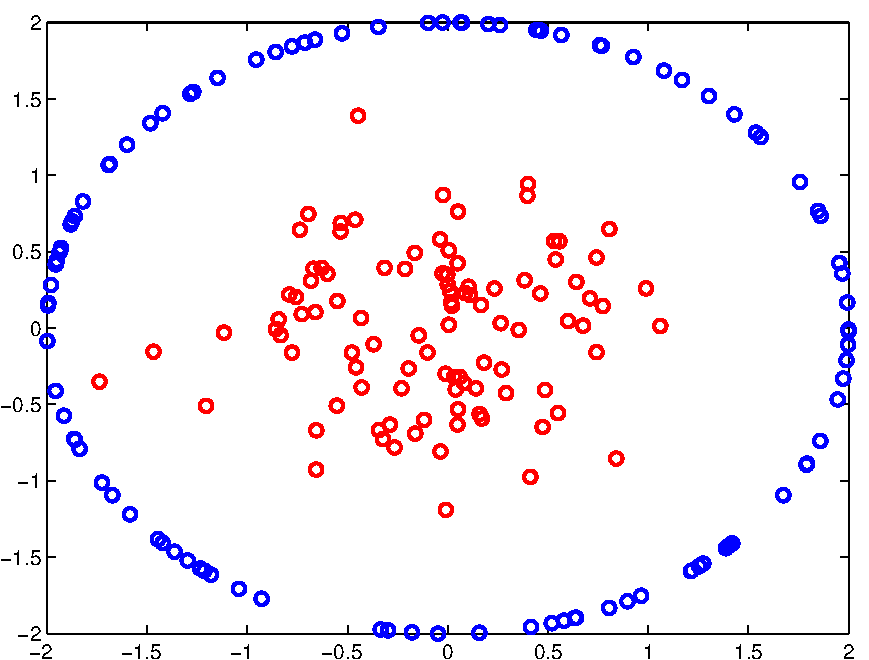
\includegraphics[width=0.45\columnwidth]{figures/pres_original_data.pdf}
    \label{fig:nlisep_data}}
     \subfloat[Linear boundary fails to separate data.]
     {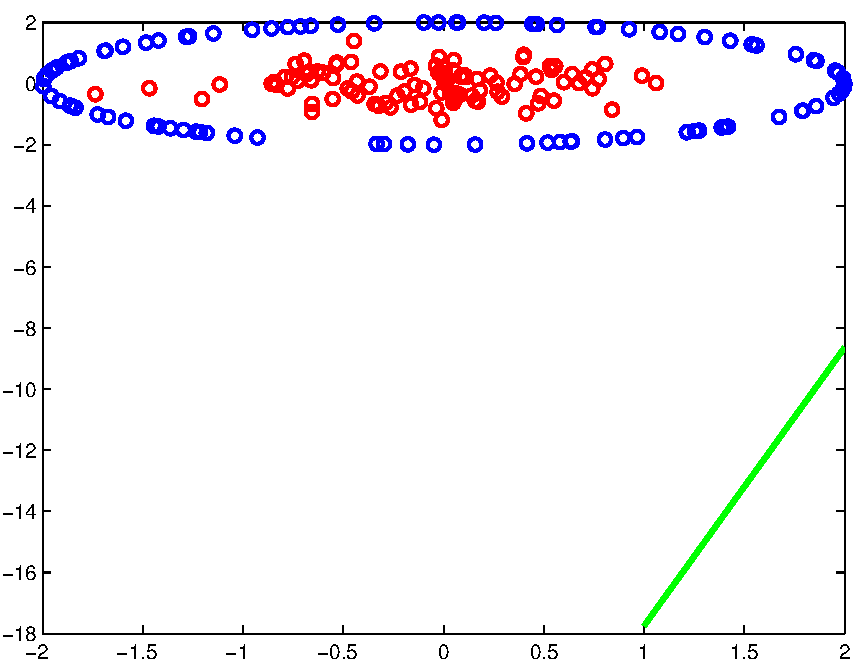
\includegraphics[width=0.45\columnwidth]{figures/pres_perc_original_data.pdf}
     \label{fig:nlin_sep_bound}}  
    \caption{Example of nonlinearly separable data. Perceptron fails to find a solution, and diverges.}
    \label{fig:nlinsep}
    %\end{figure}
%\begin{figure}[tbh] %{r}{0.5\textwidth}
\end{figure} 


\begin{figure}
\centering
    \subfloat[Nonlinear mapping of data.]
    {
    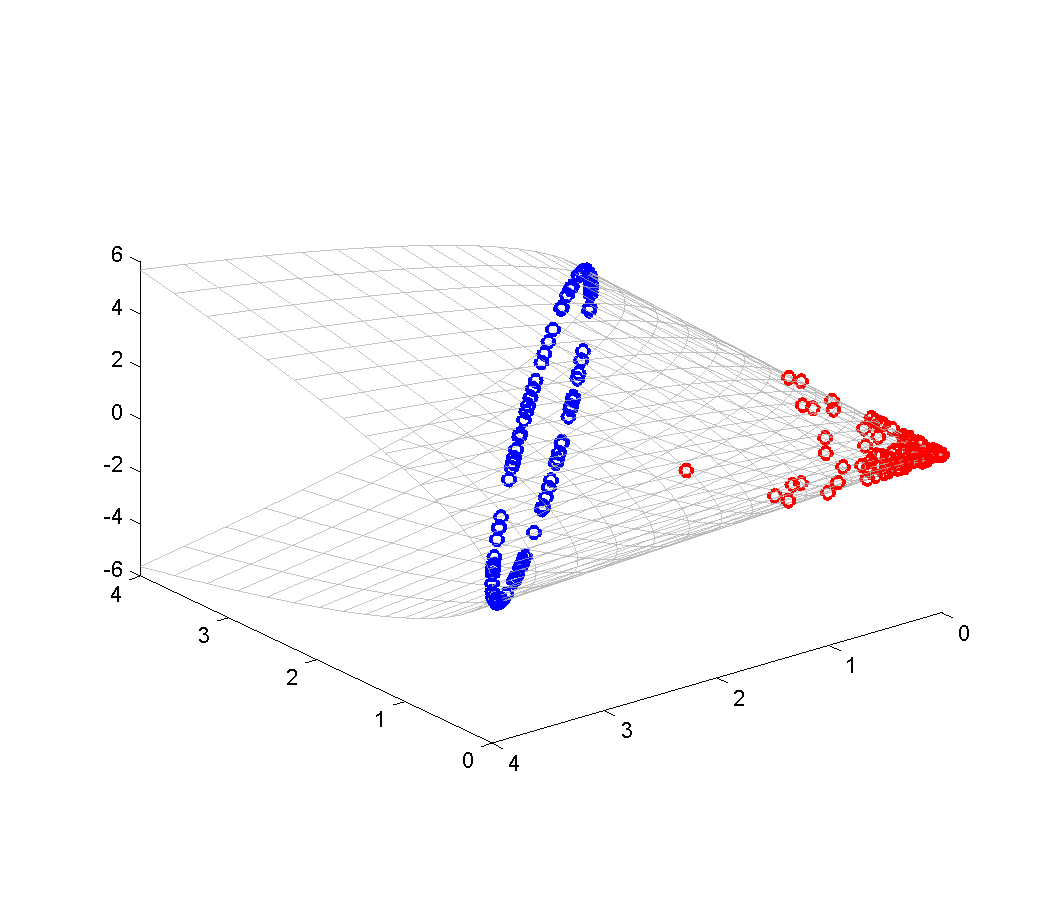
\includegraphics[width=0.45\columnwidth]{figures/fmapped_data.pdf}
    \label{fig:fmapped_data}}
     \subfloat[Linear boundary in new space.]
     {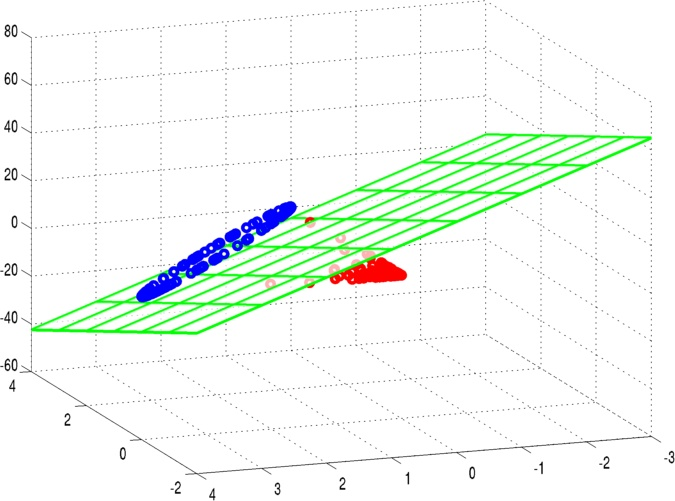
\includegraphics[width=0.45\columnwidth]{figures/pres_perc_fmapped_data_after.jpg}
     \label{fig:fmapped_bound}}  
    \caption{If we map the same data using a nonlinear map $\phi(x,y):= (x^2, y^2, 2xy)$, the perceptron now finds a solution
             in 3 dimensions.}
    \label{fig:fmapped}
    %\end{figure}
%\begin{figure}[tbh] %{r}{0.5\textwidth}
\end{figure} 